% 依固定扫描页重绘；仅示意三棱锥 S-ABC 的拓扑、点 D、E 的位置与截面 BDE，不按比例。
% 卷面图 4-6-7：D 在 AC 上，E 在 SC 上，AC 为底面内被遮挡的棱，DE 为截面与面 SAC 的交线。
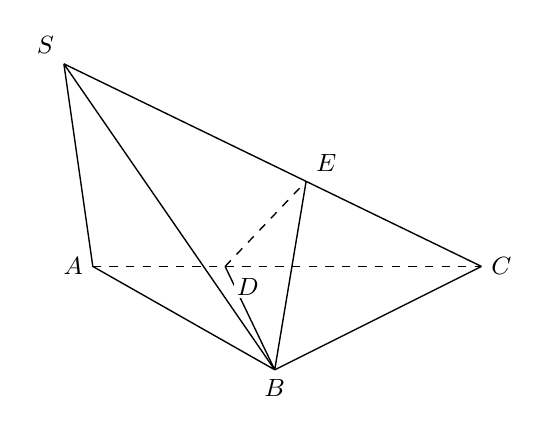
\begin{tikzpicture}[line width=.5pt,scale=1.05,font=\small]
  \coordinate (S) at (1.00,4.15);
  \coordinate (A) at (1.35,1.70);
  \coordinate (C) at (6.05,1.70);
  \coordinate (B) at (3.55,0.45);
  \coordinate (D) at (2.95,1.70);
  \coordinate (E) at (3.93,2.73);
  % 可见棱。
  \draw (S)--(A) (S)--(B) (S)--(C) (A)--(B) (B)--(C);
  % 底面被遮挡的棱 AC，以及截面内的 DE。
  \draw[dashed] (A)--(C);
  \draw[dashed] (D)--(E);
  % 截面 BDE 与底面的交线 BD、截面与面 SBC 的交线 BE。
  \draw (B)--(D) (B)--(E);
  \node[above left] at (S) {$S$};
  \node[left] at (A) {$A$};
  \node[below] at (B) {$B$};
  \node[right] at (C) {$C$};
  \node[fill=white,inner sep=1pt,below right=3pt] at (D) {$D$};
  \node[above right] at (E) {$E$};
\end{tikzpicture}
